\section{Aufbau und Durchführung}
\label{sec:Durchführung}
In einem ungeladenen , vertikal ausgerichteten Plattenkondensator wird Öl fein
zerstäubt. Diese werden mit einer Halogenlampe angestrahlt, damit dessen Bewegung
unter einem Mikroskop besser verfolgt werden können. Die angelegte Spannung kann mit
einem Multimeter gemessen werde und auch der Widerstand. Das elektrische Feld kann 
mit einem Hebel verstellt werden. Die Temperatur kann mit dem gemessenen Widerstand 
und einer Thermistor-Widerstandstabelle(\ref{fig:Abb_3}) bestimmt werden.\\
Der beschriebene Aufbau ist in \autoref{fig:Abb_2} dargestellt.
\begin{figure}[H]
    \centering
    \includegraphics[width=0.5\textwidth]{Abbildungen/Abb_2.png}
    \caption {Schematische Darstellung der Kräfte in einem homogenen elektrischen Feld\cite[1]{V503}.}
    \label{fig:Abb_2}
\end{figure}
Wie in \autoref{sec:Theorie} beschrieben werden teilweise die Öltröpfchen durch das Zerstäuben 
elektrisch geladen. Ist ein messbares Tröpfchen vorhanden, wird die Zeit gemessen, die 
das Tröpfchen benötigt eine selber gewählte Strecke zu durchlaufen.
Es wird einmal $t_0$ gemessen, wo das Teilchen ohne Einfluss des elektrischen Feldes fällt.
Anschließend wird drei mal die Steigzeit $t_{auf}$ und drei mal die Fallzeit $t_{ab}$ von 
dem gleichen Tröpfchen gemessen. Die gemessen Zeiten werden in eine Tabelle eingetragen.\\
Die Messung wird für fünf Tröpfchen durchgeführt für fünf verschiedene Spannungen.
\begin{figure}[H]
    \centering
    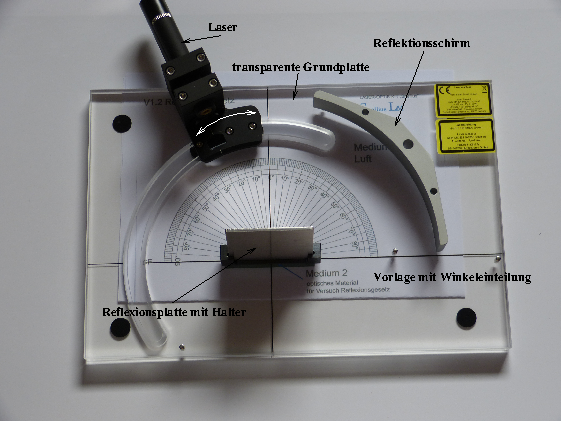
\includegraphics[width=0.5\textwidth]{Abbildungen/Abb_3.png}
    \caption {Schematische Darstellung der Kräfte in einem homogenen elektrischen Feld\cite[1]{V503}.}
    \label{fig:Abb_3}
\end{figure}